\documentclass{scrartcl}

\usepackage{amssymb}
\usepackage{amsmath}
\usepackage{mathabx}
\usepackage{tikz}
\usetikzlibrary{calc,intersections,through,backgrounds,patterns}
\usetikzlibrary{decorations.text, decorations.markings, fit}

%Source: Matthews, R. (1995). “The man who played God with infinity.” The New Scientist 147, p. 36-40
%https://www.newscientist.com/article/mg14719934-300-the-man-who-played-god-with-infinity/

\begin{document}
	
	%\begin{figure}
	%	\centering
	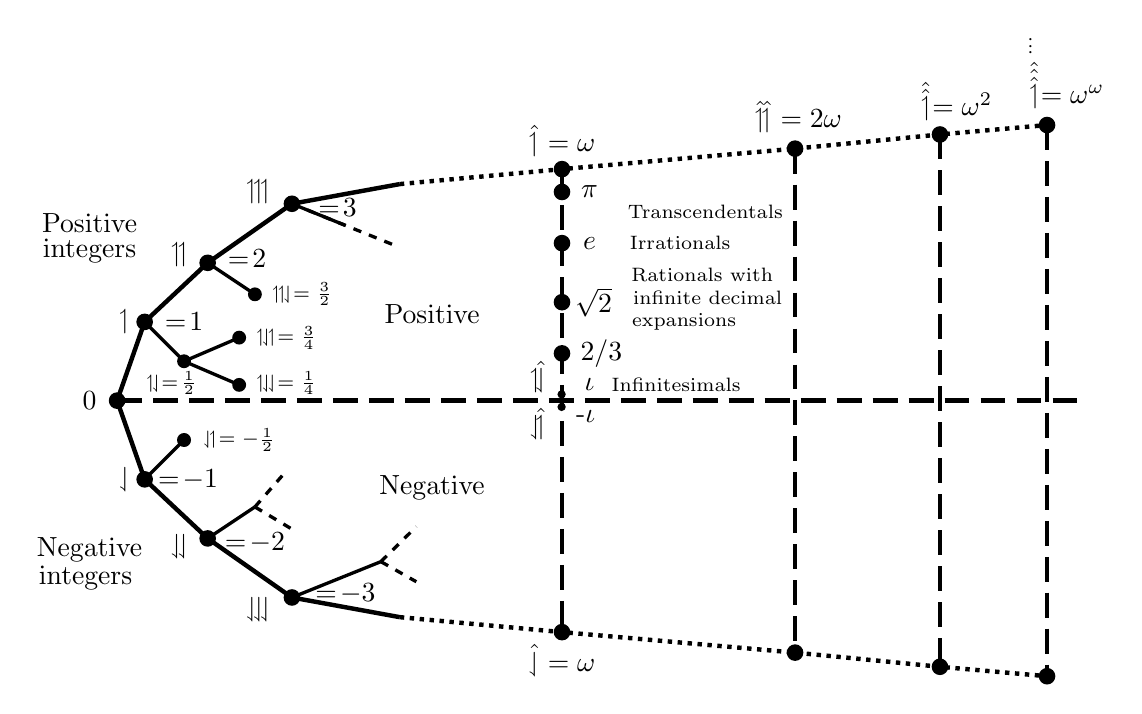
\begin{tikzpicture}
	
	\coordinate (O) at (0,0);
	\fill (O) circle (3pt);	\node at (-0.35,0) {0};	
	\draw[ultra thick,dash pattern=on 9pt off 4pt] (O)--(12.25,0);
	
	%upper dots
	\coordinate (A) at (0.35,1);		\fill (A) circle (3pt);
	\coordinate (B) at (1.15,1.75);		\fill (B) circle (3pt);
	\coordinate (C) at (2.22,2.5);		\fill (C) circle (3pt);
		\coordinate (c) at (3.59,2.75);	%transition to dotted line
	\coordinate (D) at (5.65,2.94);		\fill (D) circle (3pt);
	\coordinate (E) at (8.61,3.2);		\fill (E) circle (3pt);
	\coordinate (F) at (10.45,3.38);		\fill (F) circle (3pt);
	\coordinate (G) at (11.81,3.5);		\fill (G) circle (3pt);
	
	%\draw[ultra thick] (3.59,2.75)--(3.59,-2.75);		%testing (c)--(v)
	%\draw[ultra thick] (2.22,2.5)--(2.22,-2.5);		%testing (C)--(V)
	
	%(C) should be between ticks 5 and 6
	%(c) should be at the end of tick 8
	%(D) should be in the middle of tick 13
	%(E) should be between ticks 19 and 20
	%(F) should be between ticks 23 and 24
	%(G) should be between ticks 26 and 27
	
	%upper captions
	\node at (0.1,1) 	{$\upharpoonleft$};
	\node at (0.8,1.85) {$\upharpoonleft\!\upharpoonleft$};
	\node at (1.8,2.65) {$\upharpoonleft\!\upharpoonleft\!\upharpoonleft$};
	\node at (5.65,3.3) {$\hat{\upharpoonleft} = \omega$};
	\node at (8.65,3.6) {$\hat{\upharpoonleft}\!\hat{\upharpoonleft} = 2\omega$};
	\node at (10.7,3.8) {$\hat{\hat{\!\!\!\upharpoonleft}} = \omega^2$};
	\node at (12.1,4) 	{$\hat{\hat{\hat{\!\!\!\upharpoonleft}}} = \omega^\omega$};
	\node at (11.6,4.5) {\rotatebox{270}{{\scriptsize ...}}};
	
	%mid-upper captions
	\node at (4,1.1) 	  {Positive};
	\node at (-0.35,2.25) {Positive};
	\node at (-0.35,1.9)  {integers};
	\node at (0.85,1) 	  {$=\!1$};
	\node at (1.65,1.8)   {$=\!2$};
	\node at (2.8,2.45)   {$=\!3$};
	%
	\fill (5.65,2.65) circle (3pt); \node at (6,2.65) 	 {$\pi$};
	\fill (5.65,2) 	  circle (3pt); \node at (6,2) 		 {$e$};
	\fill (5.65,1.25) circle (3pt); \node at (6.05,1.25) {$\sqrt{2}$};
	\fill (5.65,0.6)  circle (3pt); \node at (6.15,0.6)  {2/3};
	\node at (5.35,0.3) {$\upharpoonleft\!\!\!\hat{\downharpoonleft}$};
	\fill (5.645,0.08) circle (1.5pt);
	\node at (6,0.2) 	{$\iota$};
	\node at (7.1,0.2) 	{{\scriptsize Infinitesimals}};
	\node at (7.47,2.4) {{\scriptsize Transcendentals}};
	\node at (7.15,2) 	{{\scriptsize Irrationals}};
	\node at (7.43,1.6) {{\scriptsize Rationals with}};
	\node at (7.5,1.3)  {{\scriptsize infinite decimal}};
	\node at (7.2,1) 	{{\scriptsize expansions}};
	
	%upper-mid meshwork
	\fill (0.85,0.5) circle (2.5pt);  
		\node at (0.69,0.22) {{\scriptsize $\upharpoonleft\!\downharpoonleft=\!\frac{1}{2}$}};
	\fill (1.55,0.2) circle (2.5pt);
		\node at (2.15,0.22) {{\scriptsize $\upharpoonleft\!\downharpoonleft\!\downharpoonleft=\frac{1}{4}$}};
	\fill (1.55,0.8) circle (2.5pt);
		\node at (2.15,0.8) {{\scriptsize $\upharpoonleft\!\downharpoonleft\!\upharpoonleft=\frac{3}{4}$}};
	\fill (1.75,1.35) circle (2.5pt);
		\node at (2.35,1.35) {{\scriptsize $\upharpoonleft\!\upharpoonleft\!\downharpoonleft=\frac{3}{2}$}};
	\draw[very thick] (A)--(0.85,0.5)--(1.55,0.2);	%A -- 1/2 -- 3/2
	\draw[very thick] (0.85,0.5)--(1.55,0.8);		%1/2 -- 1/4
	\draw[very thick] (B)--(1.75,1.35);				%B -- 3/2
	\draw[very thick,dashed] (C)--(3.58,1.95);		%C -- below (c)
		\draw[very thick] (C)--(2.9,2.225);			%solid part
		
	%lower-mid meshwork
	\fill (0.85,-0.5) circle (2.53pt);
	%
	\draw[very thick] (0.35,-1)--(0.85,-0.5);		%T -- -1/2
	\draw[very thick] (1.15,-1.75)--(1.75,-1.35);	%U -- (-3/2)
		\draw[very thick,dashed] (1.75,-1.35)--(2.1,-0.95);
		\draw[very thick,dashed] (1.75,-1.35)--(2.25,-1.65);
	%\draw[very thick,dashed] (2.22,-2.5)--(3.58,-1.95);		%V -- above (v)
	\draw[very thick] (2.22,-2.5)--(3.35,-2.045);	%V -- past -3
		\draw[very thick,dashed] (3.35,-2.045)--(3.8,-1.6);
		\draw[very thick,dashed] (3.35,-2.045)--(3.8,-2.3);
		
	%lower dots
	\draw[ultra thick] (O)--(A)--(B)--(C)--(c);
	\draw[ultra thick,dotted] (c)--(D)--(E)--(F)--(G);
	
	\coordinate (T) at (0.35,-1);		\fill (T) circle (3pt);
	\coordinate (U) at (1.15,-1.75);	\fill (U) circle (3pt);
	\coordinate (V) at (2.22,-2.5);		\fill (V) circle (3pt);
		\coordinate (v) at (3.59,-2.75);	%transition to dotted line
	\coordinate (W) at (5.65,-2.94);	\fill (W) circle (3pt);
	\coordinate (X) at (8.61,-3.2);		\fill (X) circle (3pt);
	\coordinate (Y) at (10.45,-3.38);	\fill (Y) circle (3pt);
	\coordinate (Z) at (11.81,-3.5);	\fill (Z) circle (3pt);
	
	%lower lines
	\draw[ultra thick] (O)--(T)--(U)--(V)--(v);
	\draw[ultra thick,dotted] (v)--(W)--(X)--(Y)--(Z);
	
	%test that dotted lines are straight
	%\draw[ultra thick,red] (c)--(G);
	%\draw[ultra thick,red] (v)--(Z);
	
	%lower captions
	\node at (0.1,-1) 	 {$\downharpoonleft$};
	\node at (0.8,-1.85) {$\downharpoonleft\!\downharpoonleft$};
	\node at (1.8,-2.65) {$\downharpoonleft\!\downharpoonleft\!\downharpoonleft$};
	\node at (5.65,-3.3) {$\hat{\downharpoonleft} = \omega$};
	
	%mid-lower captions
	\node at (4,-1.1) 		{Negative};
	\node at (-0.35,-1.9) 	{Negative};
	\node at (-0.4,-2.25) 	{integers};
	\node at (0.9,-1) 	 	{$=\!-1$};
	\node at (1.75,-1.8)  	{$=\!-2$};
	\node at (2.9,-2.45) 	{$=\!-3$};
	\node at (1.55,-0.5) 	{{\scriptsize $\downharpoonleft\!\upharpoonleft = -\frac{1}{2}$}};
	%
	\fill (5.645,-0.08) circle (1.5pt);
	\node at (5.35,-0.3) 	{$\downharpoonleft\!\!\!\hat{\upharpoonleft}$};
	\node at (5.95,-0.2) 	{-$\iota$};
	
	%vertical lines
	\draw[ultra thick,dash pattern=on 9pt off 4pt] (G)--(Z);
	\draw[ultra thick,dash pattern=on 9pt off 4pt] (F)--(Y);
	\draw[ultra thick,dash pattern=on 9pt off 4pt] (E)--(X);
	\draw[ultra thick,dash pattern=on 9pt off 4pt] (D)--(W);
	
	\end{tikzpicture}
	%	\caption{...}
	%\end{figure}
	
\end{document}